\section{HTM Network}
The HTM network consists of an SDR encoder, HTM module, and an SDR decoder to decode the predictions made by the HTM. The architecture of the Temporal Memory is explained in detail below.

\subsection{Temporal Memory Architecture}
The HTM network used in the task of predicting the fault class of the system logs consists of a single Temporal Memory layer. The architecture of the whole network and the selected parameters are presented in \autoref{tab:TMparams}, where the most important parameters are the \textit{columnCount} and \textit{cellsPerColumn}, together with the synaptic parameter of \textit{activationThreshold}. 



The first two parameters specify the number of columns and the number of cells that inhabits each column. The number of columns has to match the dimension of the presynaptic input, thus the value of $256$ had to be selected. The number of cells per column determines how many unique patterns the memory can learn. If there are too few, the memory will not be able to learn enough pattern. The default value is $32$, and with experimental analysis with the number of cells of $10,42,$ and $56$ it was determined that $10$ was too few, and values above $32$ had no significant improvement. The number of active synapses was decreased from the default value of $12$ to $8$. This allowed the temporal memory to become more sensitive and able to better detect input patterns.


\begin{table}[H]
\centering
\caption{Parameters of the Temporal Memory.}
\tiny
\label{tab:TMparams}
\begin{tabularx}{\textwidth}{l p{7.5cm} l}
\toprule
Parameter & Description &  Value\\
\midrule
        columnCount & Number of columns in the temporal memory. & 256\\
        &&\\
        cellsPerColumn & Number of cells in each column. & 32\\
        &&\\
        initialPermanence & Inital permanence value of new synapses. &0.5\\
        &&\\
        connectedPerm & The threshold permanence value for a synapse to become connected. & 0.5\\
        &&\\
        minThreshold & If the number of active potential synapses is above this threshold, the dendritic branch has detected a pattern and is eligible for learning. & 15\\
        &&\\
        newSynapseCount & The maximum number of synapses that are added to a branch during learning. & 12\\
        &&\\
        permanenceInc & The permanence incremental value rewarded to synapses with both active presynaptic and postsynaptic cells. & 0.1\\
        &&\\
        permanenceDec & The value of synaptic connections get punished with if the postsynaptic cell is active but presynaptic cell is not, and vice versa. & 0.1\\
        &&\\
        activationThreshold & For a dendritic branch to become active at least this number of synapses needs to be active. & 8\\
        &&\\
        globalDecay & Decays the permanence value of synapses when it is runs. It will also remove inactive synapses with permanence value of 0 and dendritic branches with no synapses. & 0\\
        &&\\
        burnIn & BurnIn evaluates the prediction score of the temporal memory. & 1\\
        &&\\
        checkSynapseConsistency & Will preform an invariance check of the synaptic connections if True (1). & 0\\
        &&\\
        pamLength & The number of temporal steps that the memory will remain in ''Pay Attention Mode'' after the end of a sequence. With PAM mode sequences that share elements can be learned faster. & 10\\
        &&\\
        verbosity & Controls the diagnostic output. & 0 \\
\bottomrule
\end{tabularx}
\end{table}





\section{Classification Algorithm}
To be able to classify individual system logs, each labeled log is converted into a sequence. A system log $i$ is represented as the sequence $S_i$, where $S_i = [w_1, w_2, \hdots, w_n]$ and $w_j$ is the $j$'th word in that sequence. At time $t$, the $t$'th word in the sequence, $S_i^{(t)}=w_t$, is converted to a semantic SDR via the SDR encoder. The encoder converts $w_t$ to the semantic SDR by using a look up of $w_t$ in the SDR matrix, $\boldsymbol{X}$, and thus outputs $\boldsymbol{X}_t$. The output is then fed to the temporal memory. 

\begin{figure}[H]
    \centering
    \scalebox{.5}{\centering
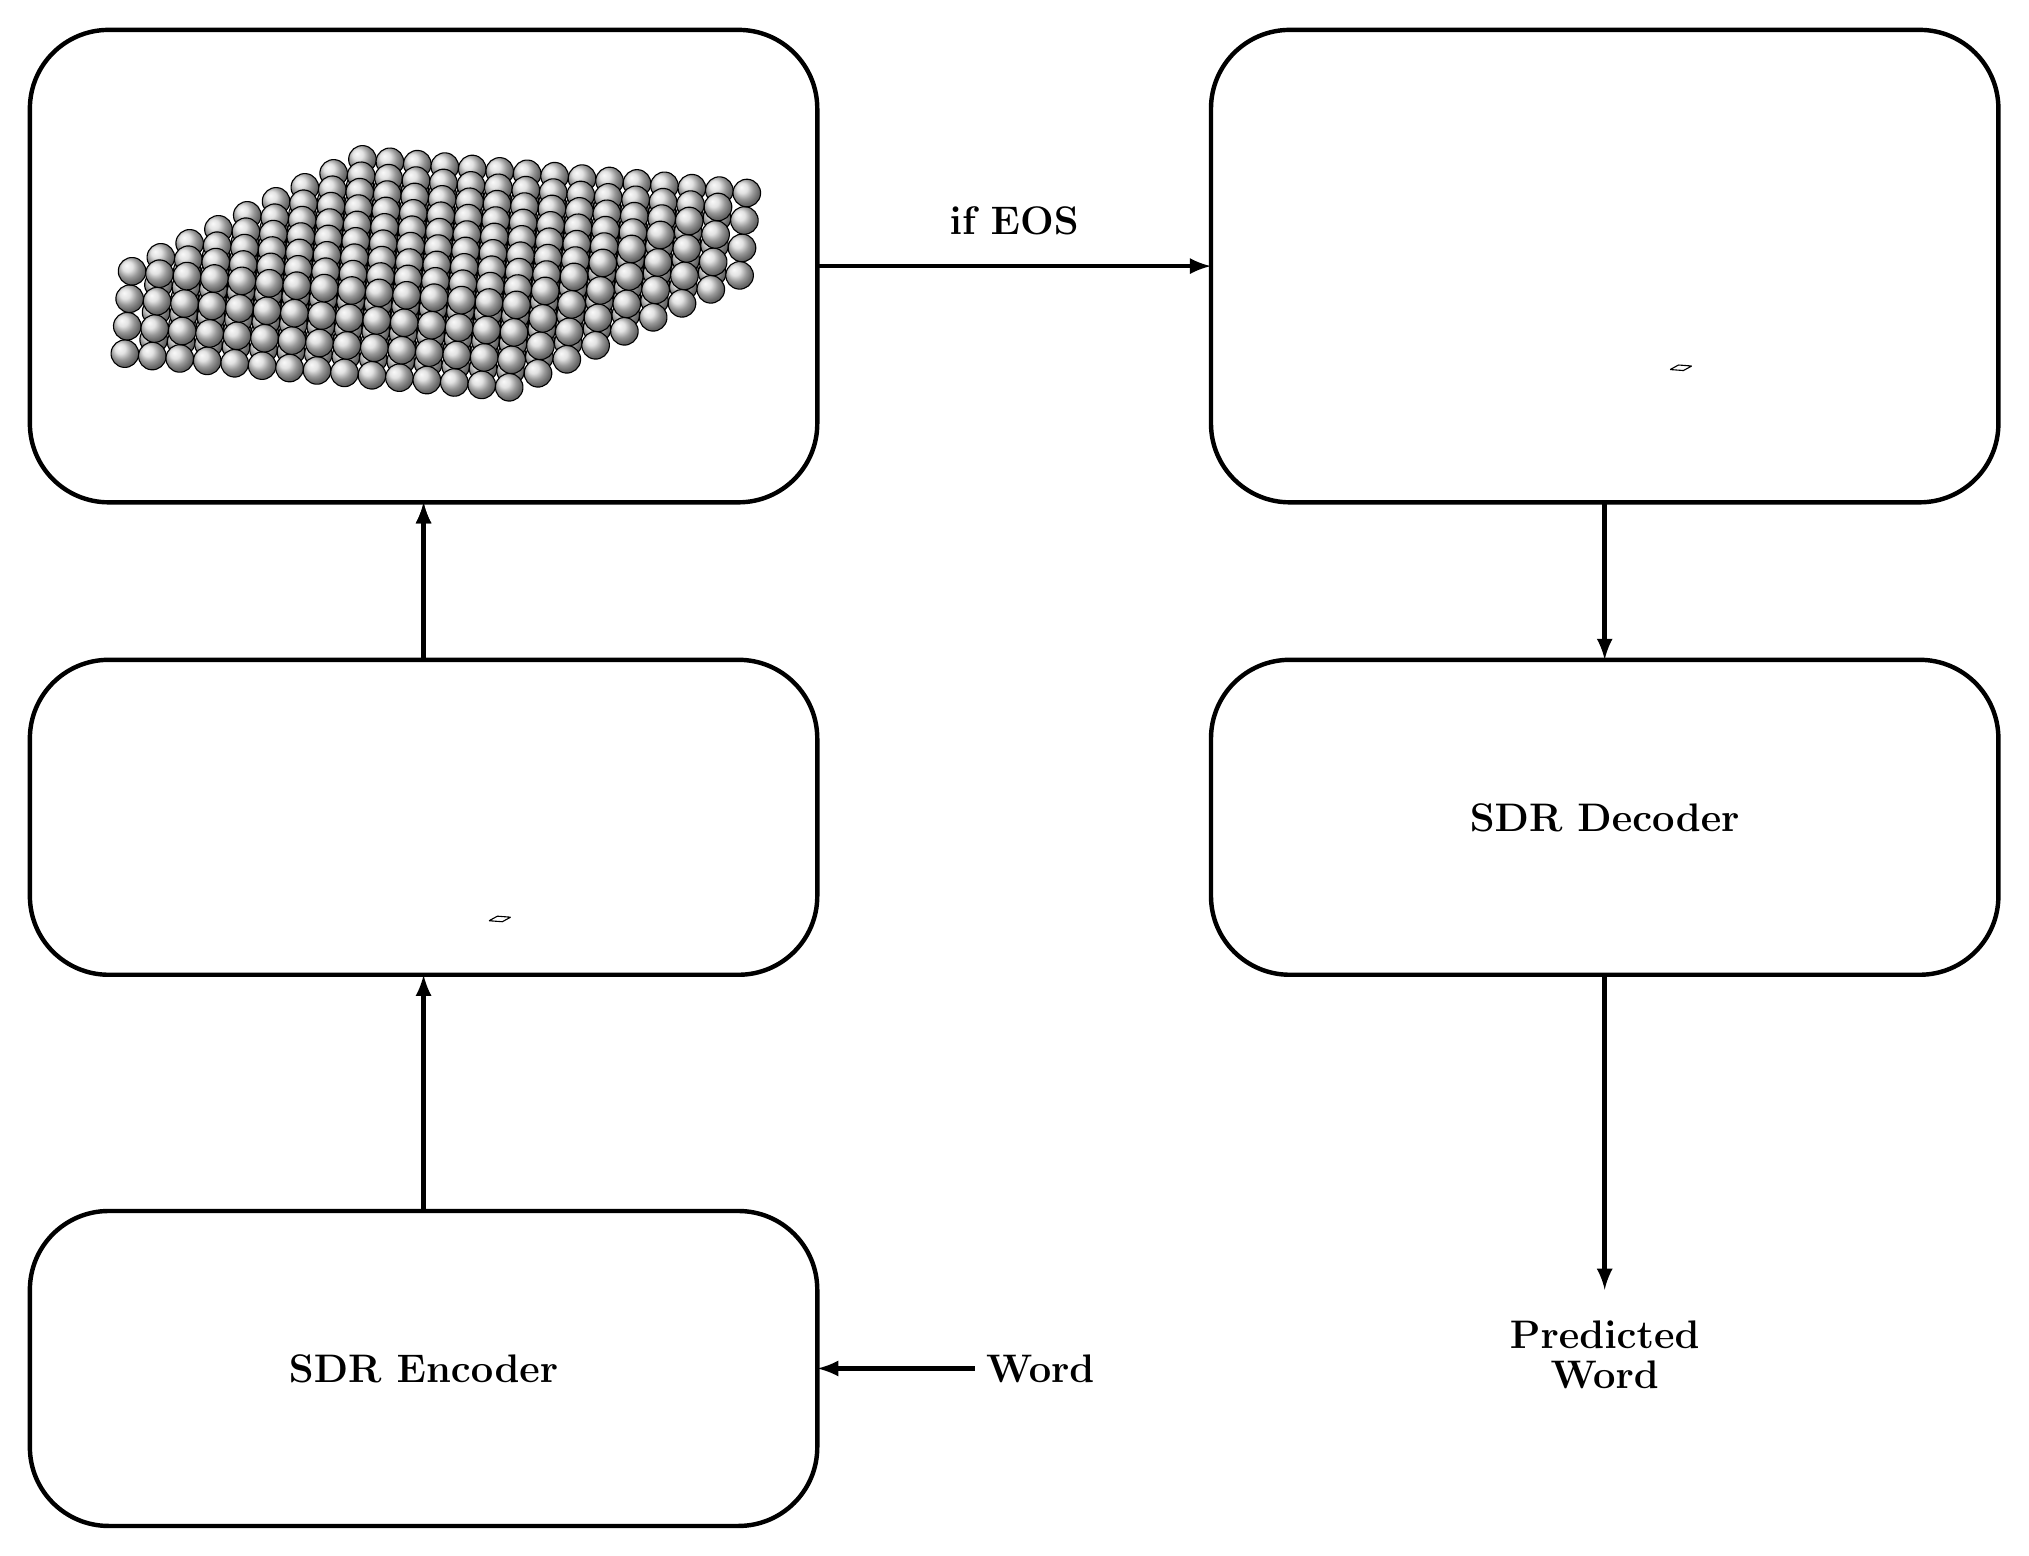
\begin{tikzpicture}



\draw[-latex,ultra thick] (6,-12) to node [right=1cm] {\Large\textbf{Word}} (4,-12);

\draw [rounded corners=1cm,ultra thick] (-6,-14) rectangle ++(10,4) node [midway] {\Large\textbf{SDR Encoder}};


\draw[-latex,ultra thick](-1,-10) to (-1,-7);



\draw [rounded corners=1cm,ultra thick] (-6,-7) rectangle ++(10,4) node [midway] {};
\begin{scope}[yshift=-180,yslant=.55,xslant=-1.6,scale=0.105]
        \ColorCells
        \draw (0, 0) grid (\GridSize, \GridSize);
        \coordinate (input);
\end{scope}

\draw[-latex,ultra thick](-1,-3) to (-1,-1);


\draw [rounded corners=1cm,ultra thick] (9,-1) rectangle ++(10,6) node [midway] {};
\begin{scope}[xshift=15cm, yshift=7cm, yshift=-180, yslant=.55, xslant=-1.6, scale=0.105] 
    \ColorCells
    \draw (0, 0) grid (\GridSize, \GridSize);
    \coordinate (output);
\end{scope}  


\draw[-latex,ultra thick](-1,-3) to (-1,-1);

\draw[-latex,ultra thick] (4,2) to node [above=.25cm] {\Large\textbf{if EOS}} (9,2);


\draw[-latex,ultra thick](14,-1) to (14,-3);

\draw [rounded corners=1cm,ultra thick] (9,-7) rectangle ++(10,4) node [midway] {\Large\textbf{SDR Decoder}};


\draw[-latex,ultra thick] (14,-7) to node [below=2.25cm] {\begin{tabular}{c} \Large\textbf{Predicted} \\ \Large\textbf{Word} \end{tabular}} (14,-11);


\draw [rounded corners=1cm,ultra thick] (-6,-1) rectangle ++(10,6) node [midway] {};

\begin{scope}[rotate around = {-5:(0,20,20)}, yshift=2.5cm,xshift=-0.5cm,scale=0.7]
   
    \foreach \x  in {0.75,1.25,1.75,2.25,2.75,3.25,3.75,4.25,4.75,5.25,5.75,6.25,6.75,7.25,7.75}%
        \shadedraw [ball color= gray!30] (\x,2,1.55*2.5) circle (0.25cm);
    \foreach \x  in {0.75,1.25,1.75,2.25,2.75,3.25,3.75,4.25,4.75,5.25,5.75,6.25,6.75,7.25,7.75}%
        \shadedraw [ball color= gray!30] (\x-.2,2,1.55*3) circle (0.25cm);
    \foreach \x  in {0.75,1.25,1.75,2.25,2.75,3.25,3.75,4.25,4.75,5.25,5.75,6.25,6.75,7.25,7.75}%
        \shadedraw [ball color= gray!30] (\x-.4,2,1.55*3.5) circle (0.25cm);
    \foreach \x  in {0.75,1.25,1.75,2.25,2.75,3.25,3.75,4.25,4.75,5.25,5.75,6.25,6.75,7.25,7.75}%
        \shadedraw [ball color= gray!30] (\x-.6,2,1.55*4) circle (0.25cm);
    \foreach \x  in {0.75,1.25,1.75,2.25,2.75,3.25,3.75,4.25,4.75,5.25,5.75,6.25,6.75,7.25,7.75}%
        \shadedraw [ball color= gray!30] (\x-.8,2,1.55*4.5) circle (0.25cm);
    \foreach \x  in {0.75,1.25,1.75,2.25,2.75,3.25,3.75,4.25,4.75,5.25,5.75,6.25,6.75,7.25,7.75}%
        \shadedraw [ball color= gray!30] (\x-1,2,1.55*5) circle (0.25cm);
    \foreach \x  in {0.75,1.25,1.75,2.25,2.75,3.25,3.75,4.25,4.75,5.25,5.75,6.25,6.75,7.25,7.75}%
        \shadedraw [ball color= gray!30] (\x-1.2,2,1.55*5.5) circle (0.25cm);
    \foreach \x  in {0.75,1.25,1.75,2.25,2.75,3.25,3.75,4.25,4.75,5.25,5.75,6.25,6.75,7.25,7.75}%
        \shadedraw [ball color= gray!30] (\x-1.4,2,1.55*6) circle (0.25cm);
    \foreach \x  in {0.75,1.25,1.75,2.25,2.75,3.25,3.75,4.25,4.75,5.25,5.75,6.25,6.75,7.25,7.75}%
        \shadedraw [ball color= gray!30] (\x-1.6,2,1.55*6.5) circle (0.25cm);


    \foreach \x  in {0.75,1.25,1.75,2.25,2.75,3.25,3.75,4.25,4.75,5.25,5.75,6.25,6.75,7.25,7.75}%
        \shadedraw [ball color= gray!30] (\x,2.5,1.55*2.5) circle (0.25cm);
    \foreach \x  in {0.75,1.25,1.75,2.25,2.75,3.25,3.75,4.25,4.75,5.25,5.75,6.25,6.75,7.25,7.75}%
        \shadedraw [ball color= gray!30] (\x-.2,2.5,1.55*3) circle (0.25cm);
    \foreach \x  in {0.75,1.25,1.75,2.25,2.75,3.25,3.75,4.25,4.75,5.25,5.75,6.25,6.75,7.25,7.75}%
        \shadedraw [ball color= gray!30] (\x-.4,2.5,1.55*3.5) circle (0.25cm);
    \foreach \x  in {0.75,1.25,1.75,2.25,2.75,3.25,3.75,4.25,4.75,5.25,5.75,6.25,6.75,7.25,7.75}%
        \shadedraw [ball color= gray!30] (\x-.6,2.5,1.55*4) circle (0.25cm);
    \foreach \x  in {0.75,1.25,1.75,2.25,2.75,3.25,3.75,4.25,4.75,5.25,5.75,6.25,6.75,7.25,7.75}%
        \shadedraw [ball color= gray!30] (\x-.8,2.5,1.55*4.5) circle (0.25cm);
    \foreach \x  in {0.75,1.25,1.75,2.25,2.75,3.25,3.75,4.25,4.75,5.25,5.75,6.25,6.75,7.25,7.75}%
        \shadedraw [ball color= gray!30] (\x-1,2.5,1.55*5) circle (0.25cm);
    \foreach \x  in {0.75,1.25,1.75,2.25,2.75,3.25,3.75,4.25,4.75,5.25,5.75,6.25,6.75,7.25,7.75}%
        \shadedraw [ball color= gray!30] (\x-1.2,2.5,1.55*5.5) circle (0.25cm);
    \foreach \x  in {0.75,1.25,1.75,2.25,2.75,3.25,3.75,4.25,4.75,5.25,5.75,6.25,6.75,7.25,7.75}%
        \shadedraw [ball color= gray!30] (\x-1.4,2.5,1.55*6) circle (0.25cm);
    \foreach \x  in {0.75,1.25,1.75,2.25,2.75,3.25,3.75,4.25,4.75,5.25,5.75,6.25,6.75,7.25,7.75}%
        \shadedraw [ball color= gray!30] (\x-1.6,2.5,1.55*6.5) circle (0.25cm);


    \foreach \x  in {0.75,1.25,1.75,2.25,2.75,3.25,3.75,4.25,4.75,5.25,5.75,6.25,6.75,7.25,7.75}%
        \shadedraw [ball color= gray!30] (\x,3,1.55*2.5) circle (0.25cm);
    \foreach \x  in {0.75,1.25,1.75,2.25,2.75,3.25,3.75,4.25,4.75,5.25,5.75,6.25,6.75,7.25,7.75}%
        \shadedraw [ball color= gray!30] (\x-.2,3,1.55*3) circle (0.25cm);
    \foreach \x  in {0.75,1.25,1.75,2.25,2.75,3.25,3.75,4.25,4.75,5.25,5.75,6.25,6.75,7.25,7.75}%
        \shadedraw [ball color= gray!30] (\x-.4,3,1.55*3.5) circle (0.25cm);
    \foreach \x  in {0.75,1.25,1.75,2.25,2.75,3.25,3.75,4.25,4.75,5.25,5.75,6.25,6.75,7.25,7.75}%
        \shadedraw [ball color= gray!30] (\x-.6,3,1.55*4) circle (0.25cm);
    \foreach \x  in {0.75,1.25,1.75,2.25,2.75,3.25,3.75,4.25,4.75,5.25,5.75,6.25,6.75,7.25,7.75}%
        \shadedraw [ball color= gray!30] (\x-.8,3,1.55*4.5) circle (0.25cm);
    \foreach \x  in {0.75,1.25,1.75,2.25,2.75,3.25,3.75,4.25,4.75,5.25,5.75,6.25,6.75,7.25,7.75}%
        \shadedraw [ball color= gray!30] (\x-1,3,1.55*5) circle (0.25cm);
     \foreach \x  in {0.75,1.25,1.75,2.25,2.75,3.25,3.75,4.25,4.75,5.25,5.75,6.25,6.75,7.25,7.75}%
        \shadedraw [ball color= gray!30] (\x-1.2,3,1.55*5.5) circle (0.25cm);
    \foreach \x  in {0.75,1.25,1.75,2.25,2.75,3.25,3.75,4.25,4.75,5.25,5.75,6.25,6.75,7.25,7.75}%
        \shadedraw [ball color= gray!30] (\x-1.4,3,1.55*6) circle (0.25cm);
    \foreach \x  in {0.75,1.25,1.75,2.25,2.75,3.25,3.75,4.25,4.75,5.25,5.75,6.25,6.75,7.25,7.75}%
        \shadedraw [ball color= gray!30] (\x-1.6,3,1.55*6.5) circle (0.25cm);
    
    
    
    \foreach \x  in {0.75,1.25,1.75,2.25,2.75,3.25,3.75,4.25,4.75,5.25,5.75,6.25,6.75,7.25,7.75}%
        \shadedraw [ball color= gray!30] (\x,3.5,1.55*2.5) circle (0.25cm);
    \foreach \x  in {0.75,1.25,1.75,2.25,2.75,3.25,3.75,4.25,4.75,5.25,5.75,6.25,6.75,7.25,7.75}%
        \shadedraw [ball color= gray!30] (\x-.2,3.5,1.55*3) circle (0.25cm);
    \foreach \x  in {0.75,1.25,1.75,2.25,2.75,3.25,3.75,4.25,4.75,5.25,5.75,6.25,6.75,7.25,7.75}%
        \shadedraw [ball color= gray!30] (\x-.4,3.5,1.55*3.5) circle (0.25cm);
    \foreach \x  in {0.75,1.25,1.75,2.25,2.75,3.25,3.75,4.25,4.75,5.25,5.75,6.25,6.75,7.25,7.75}%
        \shadedraw [ball color= gray!30] (\x-.6,3.5,1.55*4) circle (0.25cm);
    \foreach \x  in {0.75,1.25,1.75,2.25,2.75,3.25,3.75,4.25,4.75,5.25,5.75,6.25,6.75,7.25,7.75}%
        \shadedraw [ball color= gray!30] (\x-.8,3.5,1.55*4.5) circle (0.25cm);
    \foreach \x  in {0.75,1.25,1.75,2.25,2.75,3.25,3.75,4.25,4.75,5.25,5.75,6.25,6.75,7.25,7.75}%
        \shadedraw [ball color= gray!30] (\x-1,3.5,1.55*5) circle (0.25cm);
    \foreach \x  in {0.75,1.25,1.75,2.25,2.75,3.25,3.75,4.25,4.75,5.25,5.75,6.25,6.75,7.25,7.75}%
        \shadedraw [ball color= gray!30] (\x-1.2,3.5,1.55*5.5) circle (0.25cm);
    \foreach \x  in {0.75,1.25,1.75,2.25,2.75,3.25,3.75,4.25,4.75,5.25,5.75,6.25,6.75,7.25,7.75}%
        \shadedraw [ball color= gray!30] (\x-1.4,3.5,1.55*6) circle (0.25cm);
    \foreach \x  in {0.75,1.25,1.75,2.25,2.75,3.25,3.75,4.25,4.75,5.25,5.75,6.25,6.75,7.25,7.75}%
        \shadedraw [ball color= gray!30] (\x-1.6,3.5,1.55*6.5) circle (0.25cm); 
\end{scope}
\end{tikzpicture}}
    \caption{An illustration of the architecture of the classification algorithm. A word is encoded via the SDR encoder, which outputs an semantic SDR, illustrated as a gird plane, where black square represents active cells. This SDR is fed to the temporal memory layer, depicted as a stacked layers of spheres, where each sphere is an HTM neuron. If an \textit{End Of Sequence} (EOS) is reached in testing mode, the predicted SDR is extracted and decoded.}
    \label{fig:clfalg}
\end{figure}


\subsection{Training}
During training, the temporal memory uses Hebbian like learning rules to learn input sequences by forming and strengthen synaptic connections, and depressing unimportant ones. The temporal memory is only presented each sequence ones, i.e. trained using \textit{one-shot learning}. As the fault label is at the end of each sequence, represented by $w_n$, the temporal memory will be able to learn the entire sequence together with the fault label at the end. Under the training phase no decoding of predicted input SDRs is performed, which is one of the major differences in the training and testing algorithms. 


\subsection{Testing}
To test the temporal memory, the original logs are used, thus $i$'th sequence is represented $S_i^{\prime} = [w_1, w_2, \hdots, w_{n-1}]$. In the same way as during the training, each semantic SDR in the sequence is fed to the temporal memory. However, at the \textit{End Of Sequence} (EOS), as shown in \autoref{fig:clfalg}, the predicted next presynaptic input, or semantic SDR, is extracted from the temporal memory. The predicted SDR is decoded via the SDR decoder using \autoref{eq:pred}. The decoded predicted fault class of the sequence is then logged together with the actual fault label.  


\section{Metrics for Evaluation}
\label{sec:metrics}
To evaluate the HTM model we will use three different type of metrics, \textit{Confusion Matrix}, \textit{Recall}, and \textit{Accuracy}. To understand these metrics we will first introduce the following notations; \textit{True Positives}, \textit{False Positives}, \textit{True Negatives}, and \textit{False Negatives}.

\begin{itemize}
    \item \textit{True Positives} ($tp$) -- the population of sequences belonging to class $i$ that were correctly classified to be members of class $i$.
    
    \item \textit{False Positives} ($fp$) -- the population of sequences that are not members of class $i$, but were classified to belong to class $i$.
    
    \item \textit{True Negatives} ($tn$) -- the population of sequences that did not belong to class $i$ and were not classified to be members.
    
    \item \textit{False Negatives} ($fn$) -- the population of sequences that belonged to class $i$, but were classified to belong to some other class.
    
\end{itemize}



The first metric we will use for the evaluation of the HTM model is the confusion matrix, as this matrix allows us to visualise the models classification performance. In \autoref{table:conf} an illustration of the general layout of the confusion matrix is presented. 

\begin{table}

    \centering
    \renewcommand\arraystretch{1.2}
    \settowidth\rotheadsize{\theadfont Actual Class}
\caption{Illustration of a confusion metric, where $tp$ indicates correctly classified examples, and -- indicates incorrectly classified examples, if present.}
    \begin{tabular}{@{} cc ccccc}
        \toprule
        &  & \multicolumn{5}{c}{Predicted Class} \\
        &              & A & B & C & D & E \\
        \midrule
     \multirow{5}{*}[.5ex]{\rothead {Actual Class}}
        & A     & $tp$ & -- & -- & -- & --  \\
        & B     & --  & $tp$ & -- & --  & -- \\
        & C     & --  & -- & $tp$ & --  & -- \\
        & D     & --  & -- & -- & $tp$  & -- \\
        & E     & --  & -- & -- & --  & $tp$ \\
        \bottomrule
    \end{tabular}
    \label{table:conf}
\end{table}

The second metric we will use in the evaluation is called \textit{Recall}. Recall is a sensitivity metric that tells us how good a machine learning model is at correctly classifying the population of examples in class $i$. 

\begin{equation}
    Recall_i = \frac{tp_i}{tp_i + fp_i}
\end{equation}

Finally, we will evaluate the accuracy of the HTM agents classifications. Accuracy is a measure that tells us how well the algorithm is at classifying the system log examples correctly. The accuracy for class $i$ is defined as:

\begin{equation}
    Accuracy_i = \frac{tp_i + tn_i}{n}
\end{equation}

where $tp_i$ and $tn$ are the population of \textit{True Positives} and is the \textit{True Negatives} for class $i$. While $n$ is the total number of examples in the data set. However, accuracy the can be misleading if the data set is skewed, as it is in this case. For classes with few examples, the number of $tn$ will have a huge impact on the overall accuracy, as it will always be large. Accuracy is recorded to be able to compare the inference results with the Linnaeus model. 
